\hypertarget{user-interface}{%
\chapter{User Interface}\label{user-interface}}

Based on the requirements from chapter 3. Functional Requirements, it is
now possible to say something about the User Interface in general. The
main User Interface will be as implemented as a Command-line Interface.
This should be obvious after reading Chapter 3, as the chapters
requirements was written with a CLI in mind.

\hypertarget{unix-inspiration}{%
\section{Unix inspiration}\label{unix-inspiration}}

When implementing a CLI it is a good idea to draw inspiration from the
established Unix community, which has historically pushed the CLI as the
primary interface when interacting with any computer for almost any
task.

\hypertarget{unix-pipelines}{%
\subsection{\texorpdfstring{\textbf{Unix
PIpelines}}{Unix PIpelines}}\label{unix-pipelines}}

Many of the commands in the \emph{did-cli}, is designed in a way to
easily integrate with existing Unix tools. The most important part of
this integration, is to support optionally reading input from
\emph{stdin}. Also it is important to take care in how output is written
to \emph{stdout}, to make it possible to chain commands together. This
is the reason you will see that most of commands are standardized to
write full \emph{dcem}-messages to \emph{stdout}, for easy consumption
by the next command in the pipeline.

\begin{lstlisting}[language=bash]
cat message.dcem | did read | grep jonas
\end{lstlisting}

\hypertarget{unix-files}{%
\subsection{Unix Files}\label{unix-files}}

The standard usage \emph{stdin} and \emph{stdout} also makes it really
easy to work with files if necessary. Below is an example of doing the
exact same thing as in Section 4.1.1, but with files instead.

\begin{lstlisting}[language=bash]
did read message.dcem > message.dpem
grep jonas message.dpem
\end{lstlisting}

Different Unix-workflows require the ability to use both of the methods
depicted in Chapter 4.1.1 and 4.1.2, which makes it important to support
both of them. A Unix user will expect any CLI to work with both FILES
and PIPES.

\hypertarget{commands}{%
\section{Commands}\label{commands}}

This section gives a short description of all available commands in the
user interface and a screenshot of running the command.

\hypertarget{did-help}{%
\subsection{did help}\label{did-help}}

\begin{itemize}
\item
  Lists all available commands.

  \begin{figure}
  \centering
  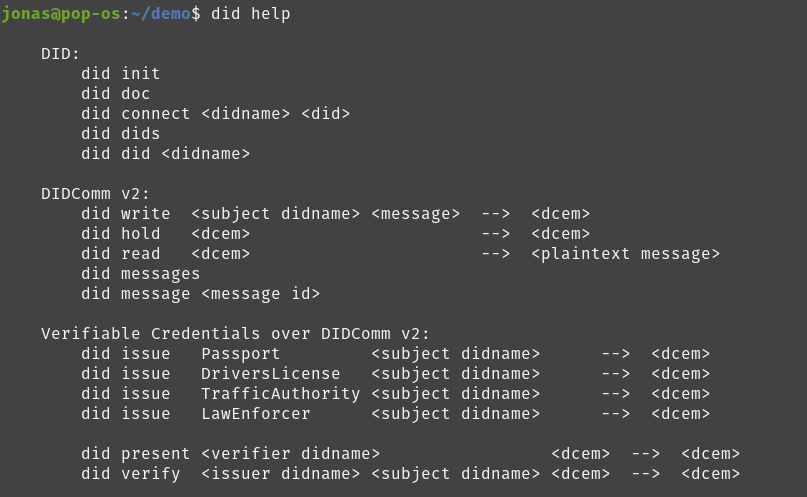
\includegraphics{User Interface f8759a9462b24d5f95cf6123d68b89ea/Untitled.png}
  \caption{Untitled}
  \end{figure}
\end{itemize}

\hypertarget{did-init}{%
\subsection{did init}\label{did-init}}

\begin{itemize}
\tightlist
\item
  Creates an agent in the current directory.
\item
  The command creates a new \passthrough{\lstinline!.did/!}directory,
  inside your working directory.
\item
  Your agents DID will be returned to \passthrough{\lstinline!stdout!}
  when running this command.
\item
  The command is idempotent.
\item
  \emph{did init} bahaves almost identical to \emph{git init.} This is
  intentional.
\end{itemize}

\begin{figure}
\centering
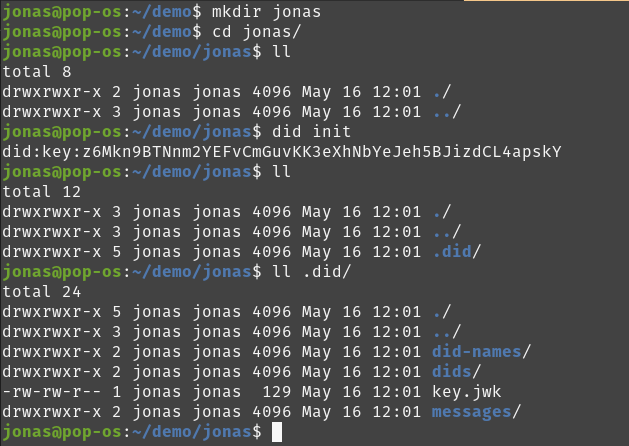
\includegraphics{User Interface f8759a9462b24d5f95cf6123d68b89ea/Untitled 1.png}
\caption{Untitled}
\end{figure}

\hypertarget{did-doc}{%
\subsection{did doc}\label{did-doc}}

\begin{itemize}
\item
  Prints the did-document, controlled by the did agent.
\item
  Since the did-agent uses did-key as it's underlying did-method, the
  did-document is generated from the public-private keypair.
\item
  Another way to describe this is that did-key is self-resolving - the
  did-document is resolved directly from the did.
\item
  This is a limitation of the did-key method, and how it is specified.
\item
  Once created, the did-document pinned to a did-key did, is not
  possible to edit.

  \begin{figure}
  \centering
  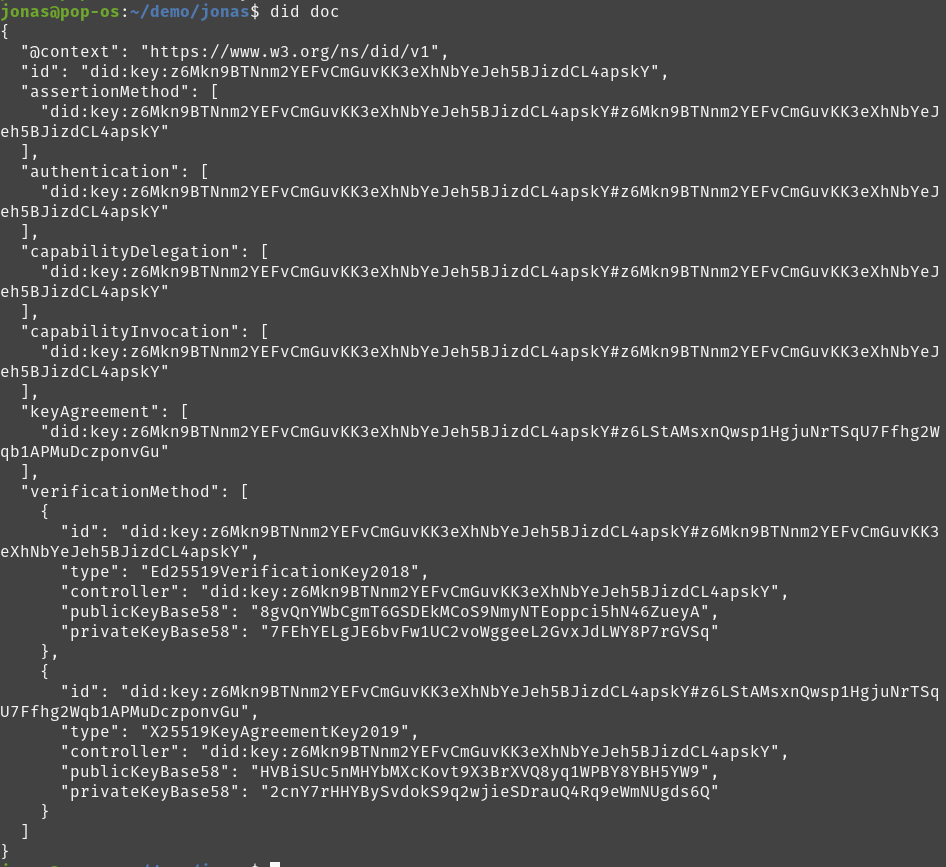
\includegraphics{User Interface f8759a9462b24d5f95cf6123d68b89ea/Untitled 2.png}
  \caption{Untitled}
  \end{figure}
\end{itemize}

\hypertarget{did-dids}{%
\subsection{did dids}\label{did-dids}}

\begin{itemize}
\item
  List all dids stored in the agent.

  \begin{figure}
  \centering
  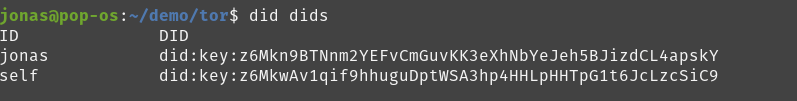
\includegraphics{User Interface f8759a9462b24d5f95cf6123d68b89ea/Untitled 3.png}
  \caption{Untitled}
  \end{figure}
\end{itemize}

\hypertarget{did-did}{%
\subsection{\texorpdfstring{did did }{did did }}\label{did-did}}

\begin{itemize}
\item
  Show the did of a single \passthrough{\lstinline!<didname>!}.

  \begin{figure}
  \centering
  
\includegraphics{User Interface f8759a9462b24d5f95cf6123d68b89ea/Untitled 4.png}
  \caption{Untitled}
  \end{figure}
\end{itemize}

\hypertarget{did-connect}{%
\subsection{\texorpdfstring{did connect
}{did connect  }}\label{did-connect}}

\begin{itemize}
\item
  \passthrough{\lstinline!did connect!} connects a
  \passthrough{\lstinline!<didname>!} to \passthrough{\lstinline!<did>!}
\item
  \passthrough{\lstinline!did connect!} gives a
  \passthrough{\lstinline!<did>!} a \passthrough{\lstinline!<didname>!}.
\item
  The \passthrough{\lstinline!<didname>!} is used in other commands, as
  an easy way to refer to another agent's
  \passthrough{\lstinline!<did>!}.

  \begin{figure}
  \centering
  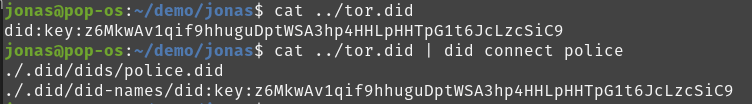
\includegraphics{User Interface f8759a9462b24d5f95cf6123d68b89ea/Untitled 5.png}
  \caption{Untitled}
  \end{figure}
\end{itemize}

\hypertarget{did-write}{%
\subsection{\texorpdfstring{did write }{did write  }}\label{did-write}}

\begin{itemize}
\item
  Wraps a user defined message inside a
  \passthrough{\lstinline!<dcem>!}envelope.
\item
  Sets the \passthrough{\lstinline!to!}header of the
  \passthrough{\lstinline!<dcem>!} to the underlying
  \passthrough{\lstinline!<did>!} refered to by the
  \passthrough{\lstinline!<didname>!}.
\item
  Gives the message a new globally unique \passthrough{\lstinline!id!} -
  GUID.

  \begin{figure}
  \centering
  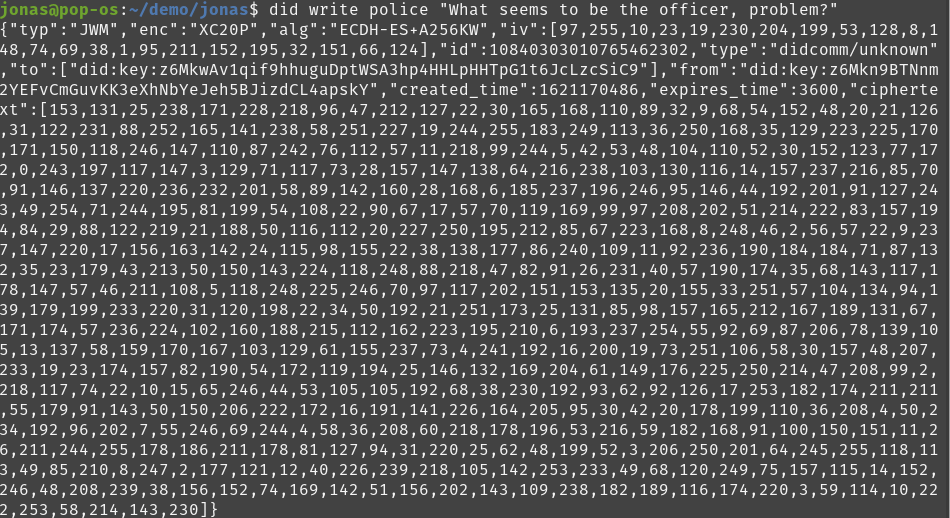
\includegraphics{User Interface f8759a9462b24d5f95cf6123d68b89ea/Untitled 6.png}
  \caption{Untitled}
  \end{figure}
\end{itemize}

\hypertarget{did-read}{%
\subsection{\texorpdfstring{did read }{did read }}\label{did-read}}

\begin{itemize}
\item
  Unwraps an \passthrough{\lstinline!<dcem>!} message from
  \passthrough{\lstinline!stdin!} or from
  \passthrough{\lstinline!<dcem>!}arg.
\item
  Prints the plaintext body of the message.
\item
  \emph{Example - Read plain message:}

  \begin{figure}
  \centering
  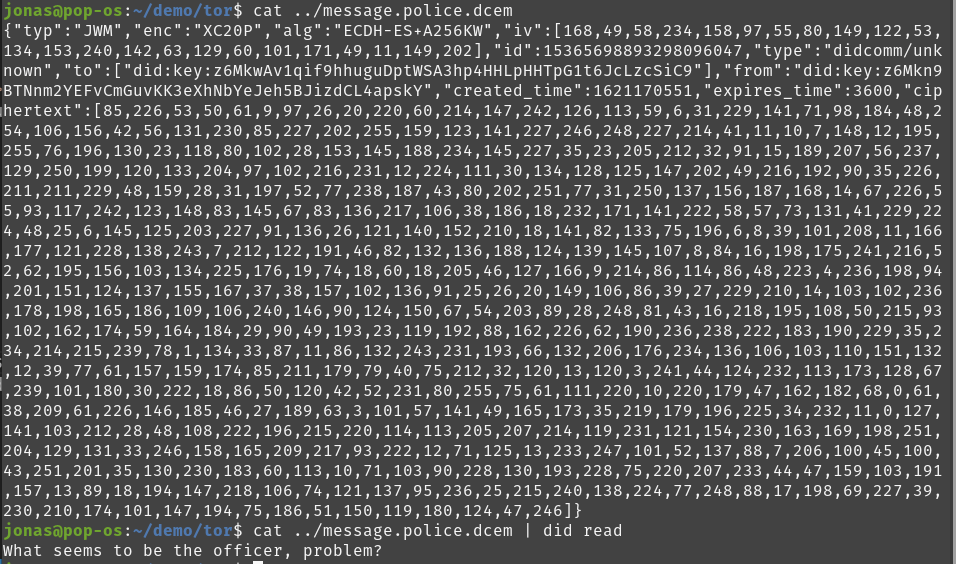
\includegraphics{User Interface f8759a9462b24d5f95cf6123d68b89ea/Untitled 7.png}
  \caption{Untitled}
  \end{figure}
\item
  \emph{Example - Read Verifiable Credential of type Passport}

  \begin{figure}
  \centering
  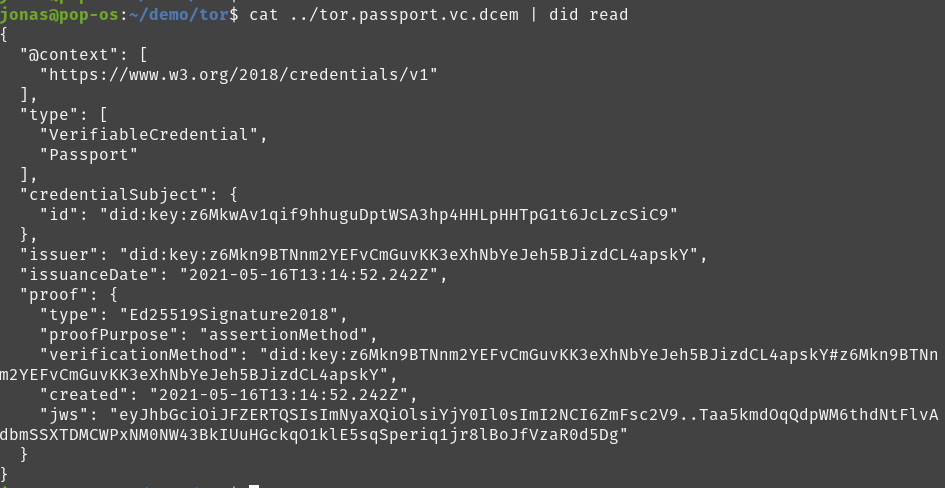
\includegraphics{User Interface f8759a9462b24d5f95cf6123d68b89ea/Untitled 8.png}
  \caption{Untitled}
  \end{figure}
\item
  Example - Read Verifiable Presentation of type Passport

  \begin{figure}
  \centering
  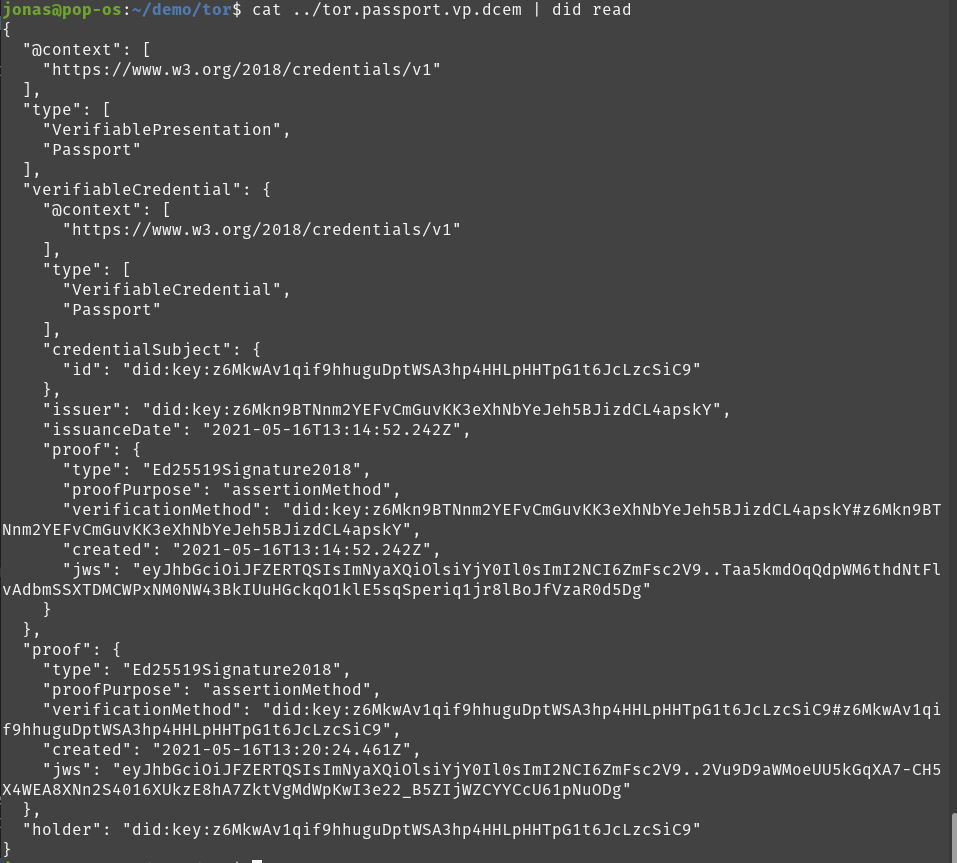
\includegraphics{User Interface f8759a9462b24d5f95cf6123d68b89ea/Untitled 9.png}
  \caption{Untitled}
  \end{figure}
\end{itemize}

\hypertarget{did-issue}{%
\subsection{\texorpdfstring{did issue }{did issue  }}\label{did-issue}}

\begin{itemize}
\item
  Issues a verifiable credential addressed to the
  \passthrough{\lstinline!did!} of \passthrough{\lstinline!<didname>!}:
\item
  Issues one of 4 \passthrough{\lstinline!<CredentialType>!}s:

  \begin{itemize}
  \tightlist
  \item
    Passport
  \item
    DriversLicense
  \item
    TrafficAuthority
  \item
    LawEnforcer
  \end{itemize}
\item
  Example of issuing a Verifiable Credential of type Passport

  \begin{figure}
  \centering
  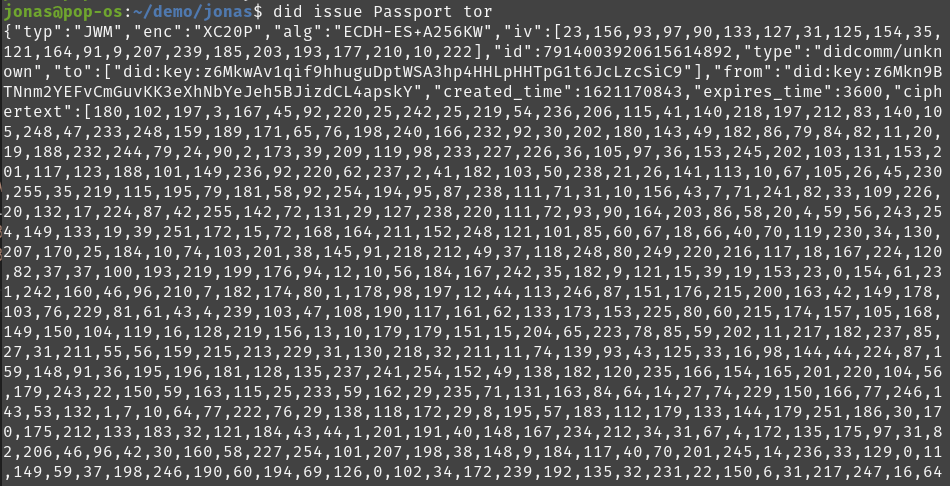
\includegraphics{User Interface f8759a9462b24d5f95cf6123d68b89ea/Untitled 10.png}
  \caption{Untitled}
  \end{figure}
\end{itemize}

\hypertarget{did-hold}{%
\subsection{\texorpdfstring{did hold }{did hold }}\label{did-hold}}

\begin{itemize}
\item
  Holds and prints it to stdout

  \begin{figure}
  \centering
  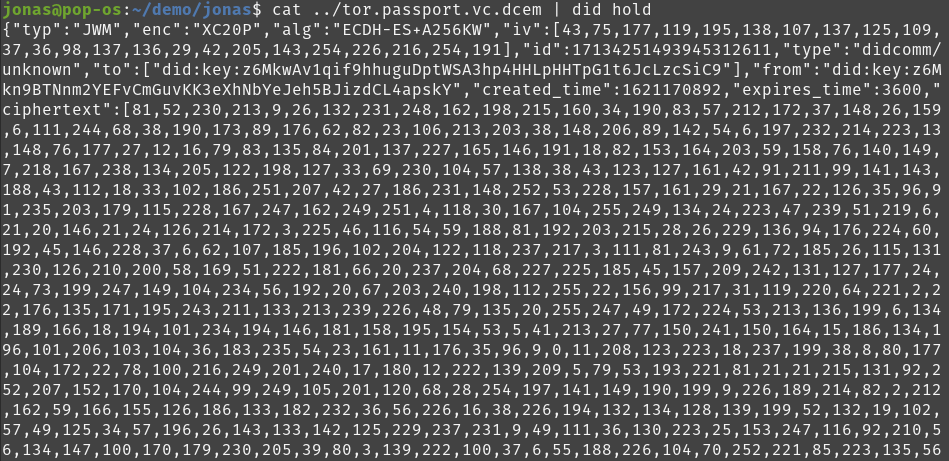
\includegraphics{User Interface f8759a9462b24d5f95cf6123d68b89ea/Untitled 11.png}
  \caption{Untitled}
  \end{figure}
\end{itemize}

\hypertarget{did-present}{%
\subsection{\texorpdfstring{did present
}{did present  }}\label{did-present}}

\begin{itemize}
\item
  Prints a Verifiable Presentation to stdout, with as it's content

  \begin{figure}
  \centering
  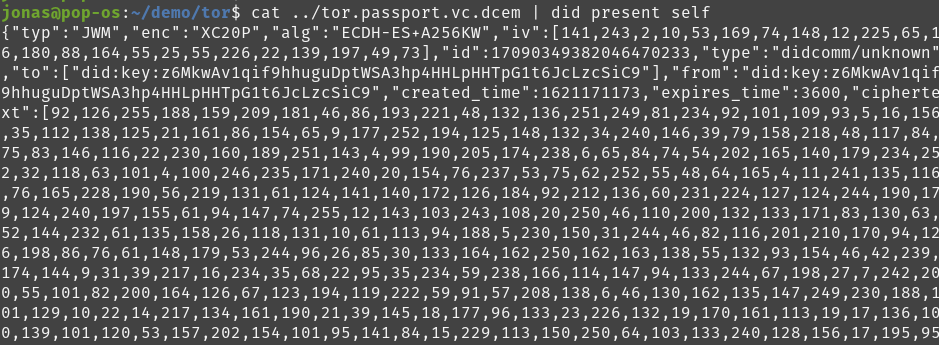
\includegraphics{User Interface f8759a9462b24d5f95cf6123d68b89ea/Untitled 12.png}
  \caption{Untitled}
  \end{figure}
\end{itemize}

\hypertarget{did-verify}{%
\subsection{\texorpdfstring{did verify
}{did verify   }}\label{did-verify}}

\begin{itemize}
\item
  Prints \passthrough{\lstinline!<dcem>!} to
  \passthrough{\lstinline!stdout!}, if, and only if, verification
  succeeds.
\item
  Example - where verification succeeds:

  \begin{figure}
  \centering
  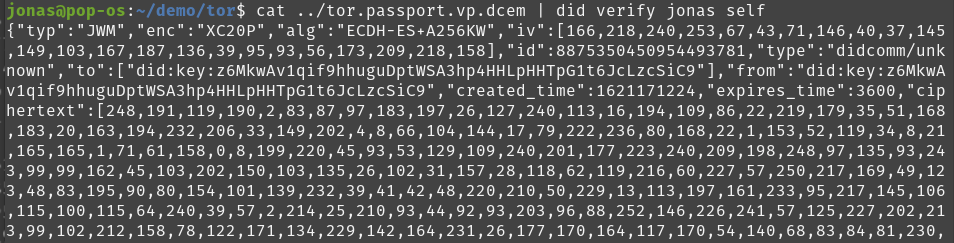
\includegraphics{User Interface f8759a9462b24d5f95cf6123d68b89ea/Untitled 13.png}
  \caption{Untitled}
  \end{figure}
\item
  Example - where verification fails:

  \begin{figure}
  \centering
  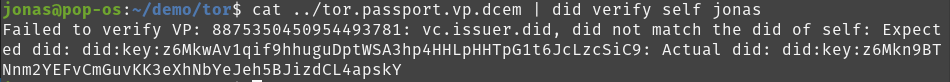
\includegraphics{User Interface f8759a9462b24d5f95cf6123d68b89ea/Untitled 14.png}
  \caption{Untitled}
  \end{figure}
\end{itemize}

\hypertarget{did-messages}{%
\subsection{did messages}\label{did-messages}}

\begin{itemize}
\item
  List all didcomm messages stored in the wallet.
\item
  Messages are added to the wallet when using the
  \passthrough{\lstinline!did hold!} command.

  \begin{figure}
  \centering
  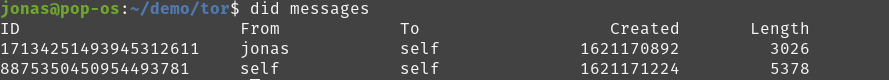
\includegraphics{User Interface f8759a9462b24d5f95cf6123d68b89ea/Untitled 15.png}
  \caption{Untitled}
  \end{figure}
\end{itemize}

\hypertarget{did-message}{%
\subsection{\texorpdfstring{did message
}{did message }}\label{did-message}}

\begin{itemize}
\item
  Show the contents of a single didcomm message based on the given
  \passthrough{\lstinline!<message id>!}.

  \begin{figure}
  \centering
  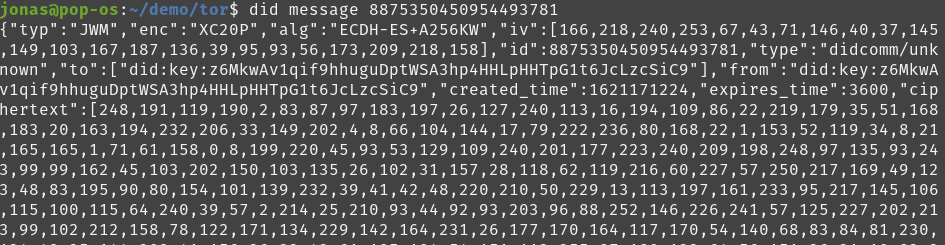
\includegraphics{User Interface f8759a9462b24d5f95cf6123d68b89ea/Untitled 16.png}
  \caption{Untitled}
  \end{figure}
\end{itemize}

\hypertarget{intentional-limitations-of-the-cli}{%
\section{Intentional limitations of the
CLI}\label{intentional-limitations-of-the-cli}}

\begin{itemize}
\tightlist
\item
  None of the commands have any optional-arguments - e.g
  \passthrough{\lstinline!-option=<arg>!}. This is to keep program logic
  as simple as possible. If the CLI was intended for a broader audicene
  with multiple use-cases, options may be added. This CLI is a special
  purpose CLI, intended to solve a specific use-case, namely the
  specific proof-of-concept from the problem statement. This is why
  optional-arguments was not prioritized.
\item
  Options are much harder to parse correctly than fixed size positional
  arguments.
\item
  None of the commands required variable length arguments, which made
  the implementation easier.
\item
  None of the commands have filepath arguments. The user is expected to
  use \passthrough{\lstinline!cat <filepath>!} to read the contents of a
  file, which is then fed into a positional argument of one of the
  commands. Example:
  \passthrough{\lstinline!did read \\\\$(cat ../message.dcem)!} vs
  \passthrough{\lstinline!did read ../message.dcem!}. This was done to
  simplify implementation.
\end{itemize}
